\documentclass[UTF8,a4paper,11pt]{article}
\usepackage{fancyhdr}
\usepackage{multicol} % 正文单双栏混排
\usepackage{lastpage} % 用于获得最大页数,页眉显示用
\usepackage{geometry} % 用于设置页边距
\usepackage[subfigure,AllowH]{graphfig} %图片相关
\usepackage{booktabs} % 导入三线表需要的宏包
\usepackage{multirow}
\usepackage{graphicx}
\usepackage{amsmath} % 导入矩阵等
\usepackage{float}%图片相关
\geometry{left=3cm,right=3.8cm,top=2.5cm,bottom=2.5cm}
%%%%%%%%%%%%%%%%%%%%%%%%%%%%%%%%%%%%%%%%%%%%%%%%%%%%%%%%%%%%%%%%
%定义行间距为1.1倍行距
\renewcommand{\baselinestretch}{1.1}
%重新定义缩进长度 pt是字号
\parindent 22pt


\fancypagestyle{plain}{
\fancyhf{}
\lhead{Oct,2023}
\chead{
\includegraphics[scale=0.5]{logo.png}}
\rhead{Page \thepage\ of \pageref{LastPage}}
\lfoot{}
\cfoot{\centering{Kangan Qian 2023210335}}
\rfoot{}
}
\pagestyle{plain}

\title{\textbf{\huge{Homework for lecture2}}}
\author{Kangan Qian
\\2023210335}
\date{} % 这一行用来去掉默认的日期显示

\begin{document}
\newcommand{\supercite}[1]{\textsuperscript{\cite{#1}}}
%%%%%%%%%%%%%%%%%%%%%%%%%%%%%%%%%%%%%%%%%%%%%%%%%%%%%%%%%%%%%%%%
% 显示title
\maketitle
\setlength{\oddsidemargin}{ 1cm} % 3.17cm - 1 inch
\setlength{\evensidemargin}{\oddsidemargin}
\setlength{\textwidth}{13.50cm}
%添加标题和摘要的距离
%vspace{…}是竖直距离
%hspace{…}是水平距离
\vspace{-0.2cm}

\section{Problem1}
\subsection{Problem1 Restatement}
Considering the background information of and limiting conditions identified in the problem statement, we are supposed to address the following problems:
\begin{itemize}
\item Let's break down the given information and understand the scenario. Imagine we have a series of experiments where a vehicle is coasting on a road with a constant slope. In these tests, there is no wind affecting the vehicle's motion. The vehicle starts at a speed of 20 meters per second and coasts until it comes to a stop while in neutral gear. The interesting part is that this process is repeated four times, with the vehicle going back and forth between two points.
\item
To analyze the data from these tests, we have two files: "data\_A2B.mat" and "data\_B2A.mat." The first file contains the data when the vehicle is coasting from point A to point B, while the second file contains the data for the coasting from point B to point A. Each file is divided into four groups of data. Within each group, we have three columns: time in seconds, vehicle velocity in meters per second, and longitudinal acceleration in meters per second squared.
\item
It's important to note that the measured data may not be completely accurate due to imperfections in the sensors used. They might introduce some biases and noise into the measurements. However, we have some known parameters available that could help us analyze the data further.


\end{itemize}
\subsection{Data Preprocess}
For the reason that the measured data may not be completely accurate due to imperfections in the sensors used. They might introduce some biases and noise into the measurements. Simple methods for rejecting outliers are applied.

\subsection{Longgitudinal Vehicle Dynamics model}
For the vehicle uphill, the equation of forces along the plane is:
\begin{equation}\label{eq1}
\sum F_x = -fm_egcos\theta-\frac{1}{2}C_DA\rho u^2-m_egcos\theta = m_ea
\end{equation}
For the vehicle downhill, the equation of forces along the plane is:
\begin{equation}\label{eq2}
\sum F_x = -fm_egcos\theta-\frac{1}{2}C_DA\rho u^2+m_egcos\theta = m_ea
\end{equation}
In the equation \ref{eq1} and \ref{eq2},$m_e$ means equivalent mass. This variable can be represented as:
$$m_e = m + \frac{\sum I_w}{r^2}$$

\subsection{Solution1:Linear Regression}
The two equations can be written as the linear function between $a$ and $u^2$:
$$
u^{2}=\frac{-m_{e} a-f m g \cos \theta-m g \sin \theta}{\frac{1}{2} C_{D} A \rho}=-\frac{2\left(m+\sum \frac{I_{W}}{r^{2}}\right)}{C_{D} A \rho} a+\frac{2(-\sin \theta-f \cos \theta)}{C_{D} A \rho} m g
$$
Let above formula represent as $$u^2=k_{1} a+b_{1}$$
$$
k_1 = -\frac{2\left(m+\sum \frac{I_{W}}{r^{2}}\right)}{C_{D} A \rho}
$$

$$
b_1 = \frac{2(-\sin \theta-f \cos \theta)}{C_{D} A \rho} m g
$$
Simlarly,we can also get another one:
$$
u^{2}=\frac{-m_{e} a-f m g \cos \theta-m g \sin \theta}{\frac{1}{2} C_{D} A \rho}=-\frac{2\left(m+\sum \frac{I_{W}}{r^{2}}\right)}{C_{D} A \rho} a+\frac{2(\sin \theta-f \cos \theta)}{C_{D} A \rho} m g
$$

Let above formula represent as $$u^2=k_{2} a+b_{2}$$
$$
k_2 = -\frac{2\left(m+\sum \frac{I_{W}}{r^{2}}\right)}{C_{D} A \rho}
$$
$$
b_2 = \frac{2(\sin \theta-f \cos \theta)}{C_{D} A \rho} m g
$$
Perform linear regression for different points in . The following are eight regression results and the figure would like to be shown in appendix.
\begin{table}[!ht]
    \centering
    \caption{Linear Regression Results}
    \begin{tabular}{lllllll}
    \toprule[1.5pt]
        ~ & ~ & Test1 & Test2 & Test3 & Test4 & Weighted-average \\ 
        \midrule[0.75pt]
        A2B & $k_1$ & -3250.5 & -3178.2 & -3193.5 & -3238.6 & -3215.2 \\ 
        ~ & $b_1$ & -795.0 & -776.2 & -780.2 & -791.6 & -785.8 \\ 
        B2A & $k_2$ & -3215.5 & -3210.5 & -3194.2 & -3197.3 & -3204.3 \\ 
        ~ & $b_2$ & -181.2 & -181.1 & -179.6 & -180.0 & -180.5 \\ 
        \bottomrule[1.5pt]
    \end{tabular}
\end{table}
The weight in the above table can be calculate by following formula,$\alpha_i$ represents the accuracy of the linear model:
\begin{equation}
\omega = \frac{\alpha_i }{\sum_{i=1}^{n} \alpha_i} ,i=1,2,3,4
\end{equation}

$$
\alpha_i = loss^{-1}
$$
Note that the slopes in equation(1) and (2) take the same form. Denote the average $k_1$ and $k_2$ as $k$. 
Then use $k$ and $b$ to calculate $C_D$:
$$
C_D = -\frac{2\left(m+\sum \frac{I_{W}}{r^{2}}\right)}{k A \rho} = 0.3589
$$
Then calculate the means of the intercepts respectively as $b_1$ and $b_2$,
$$
b_1 + b_2 = -4\frac{fcos\theta}{C_DA\rho}mg
$$

$$
b_1 - b_2 = -4\frac{sin\theta}{C_DA\rho}mg
$$

To solve these 2 equations,we get $\theta = 0.0100$,
$$
i = tan \theta = 0.010029 \quad f = 0.01601
$$

\subsection{Solution2:Paramater estimation based on Genetic Algorithm}

Consider below ODE,
\begin{equation}
 -fm_egcos\theta-\frac{1}{2}C_DA\rho u^2-m_egcos\theta = m_e\dot{u},
 u(0) = 20
\end{equation}

\begin{equation}
 -fm_egcos\theta-\frac{1}{2}C_DA\rho u^2 + m_egcos\theta = m_e\dot{u},
 u(0) = 20
\end{equation}

To estimate the parameter,we use Genetic Algorithm(GA) as the optimal method. The method flow charts are listed as follows:

  \begin{figure}[htbp]
  	\begin{minipage}[t]{0.45\linewidth}
  		\centering
  		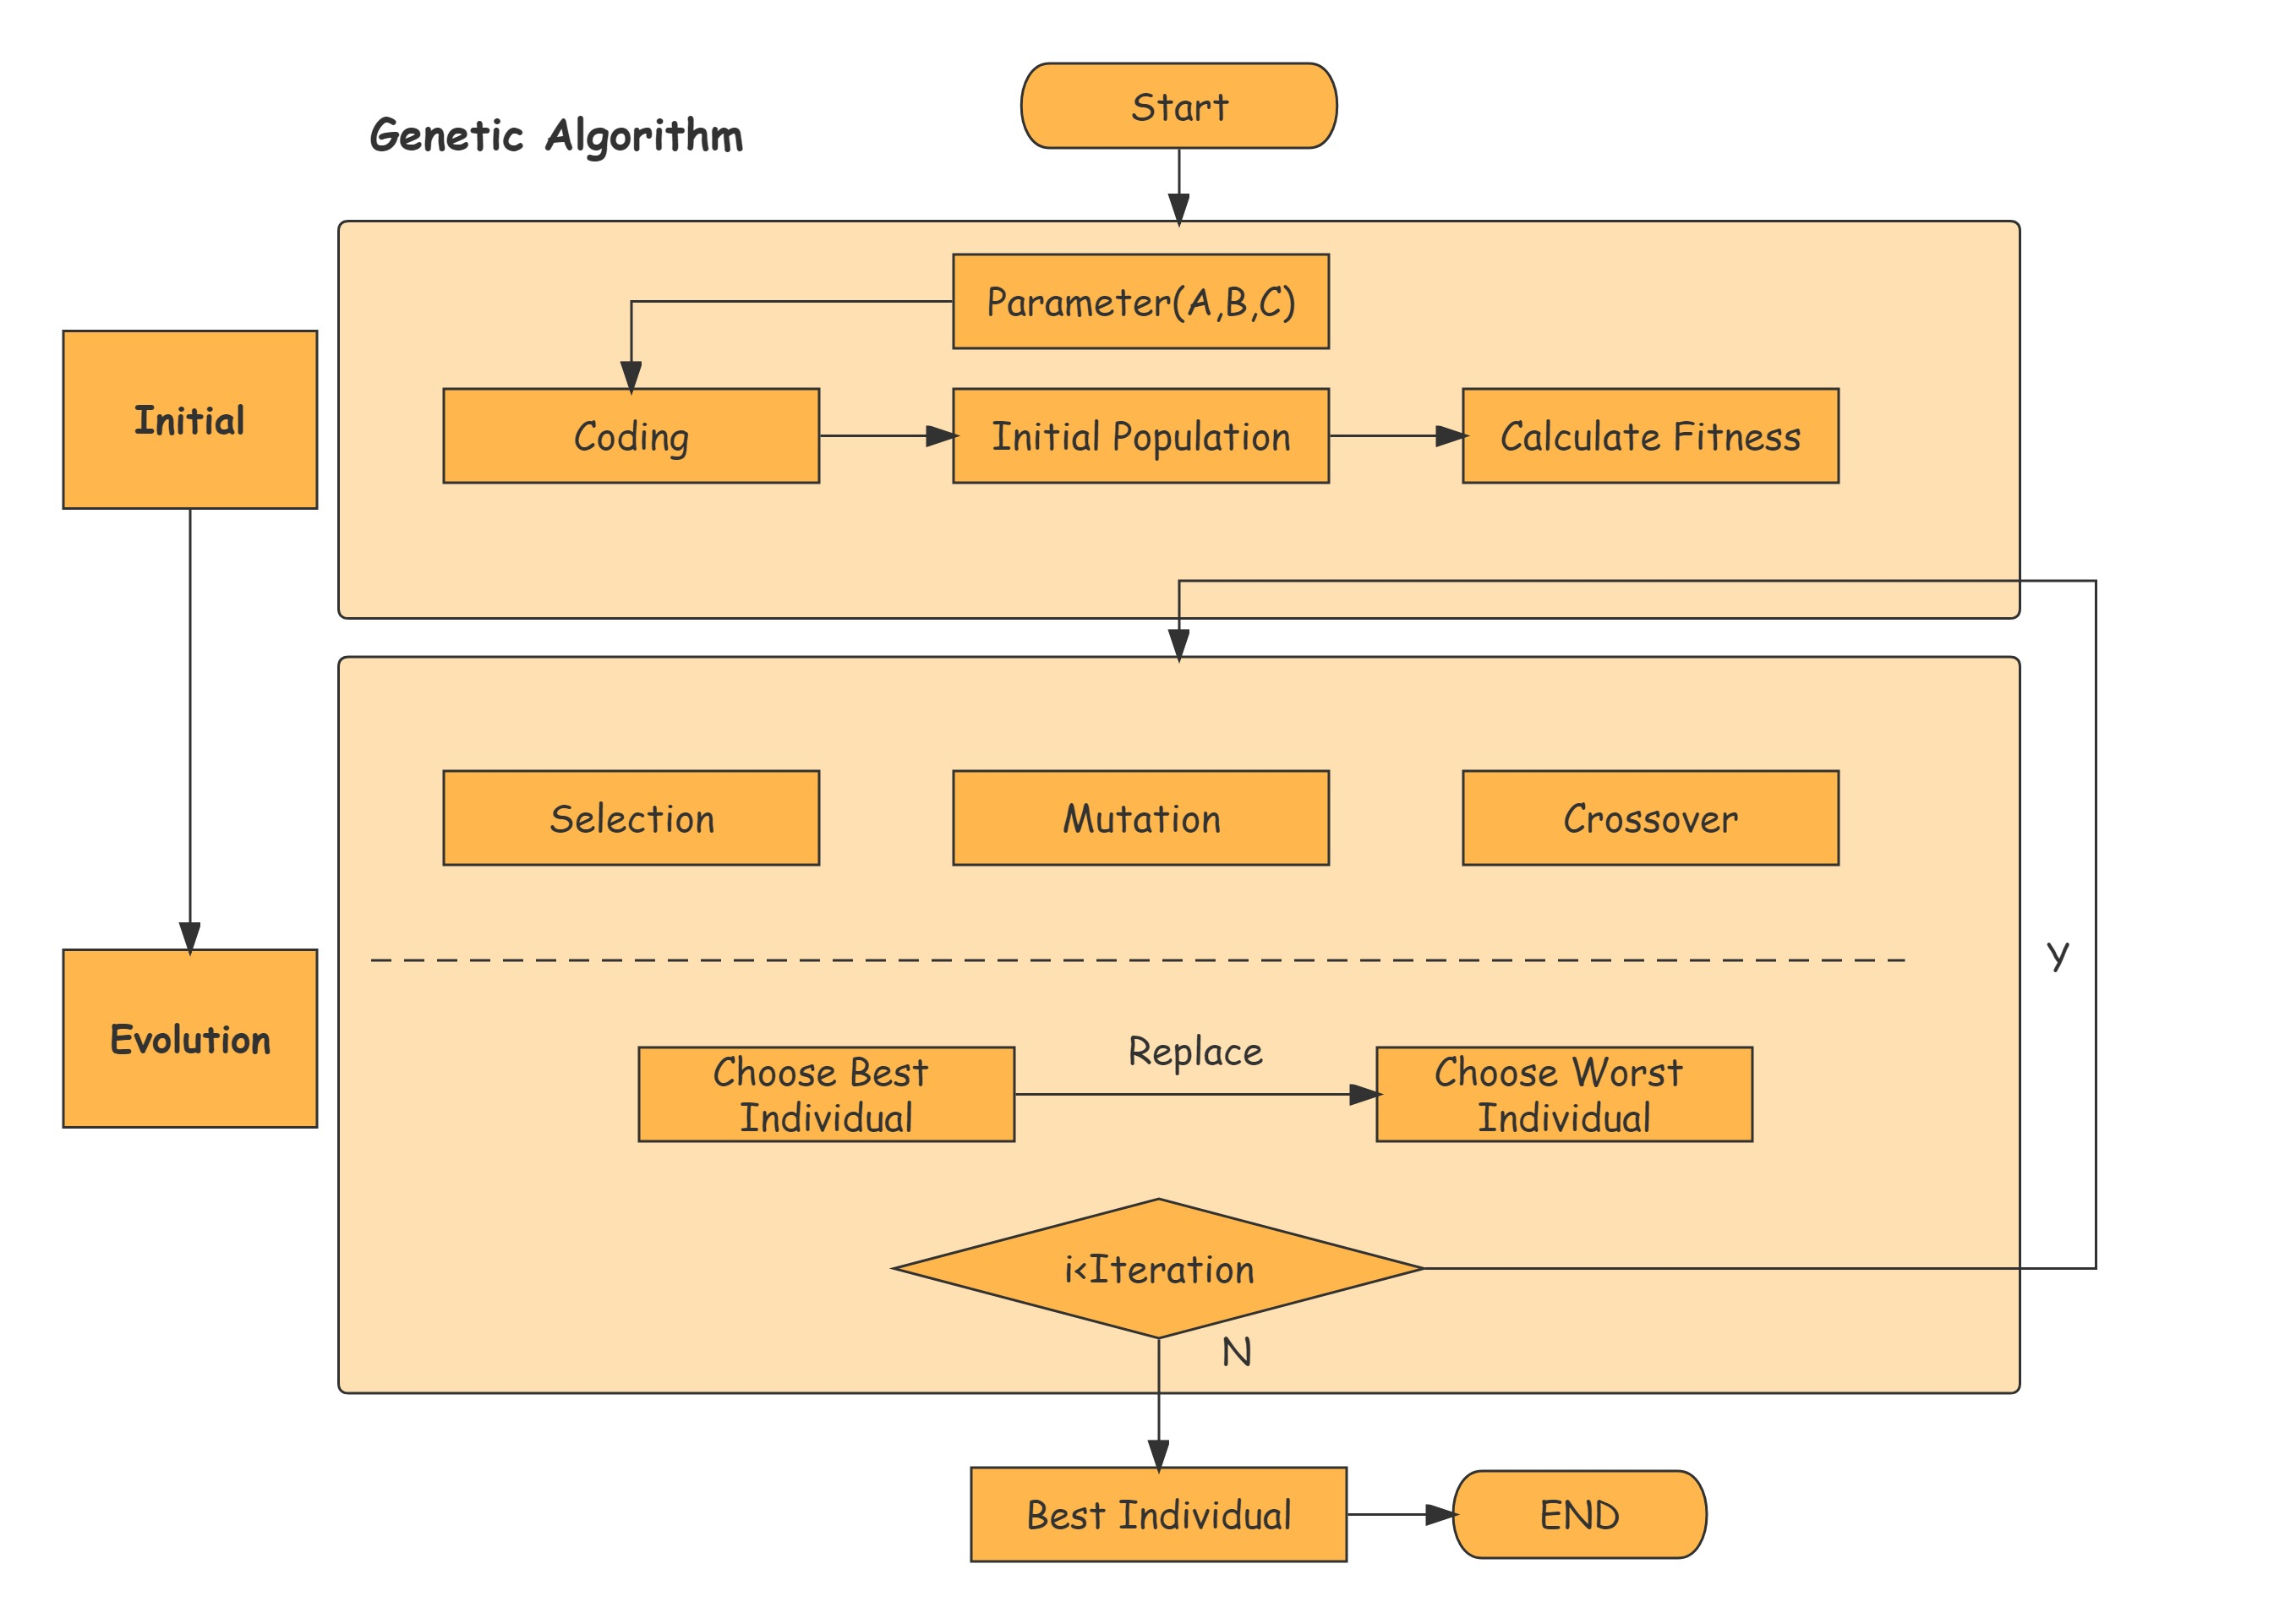
\includegraphics[width=7cm]{GA.jpg}
  		%\caption{Genetic Algorithm Steps}
  	\end{minipage}
  	\begin{minipage}[t]{0.45\linewidth}        %图片占用一行宽度的45%
  		\hspace{2mm}
  		\includegraphics[width=6cm]{GA\_bi.png}
  		%\caption{Biological Principles of Genetic Algorithms}
  	\end{minipage}
  	\caption{Genetic Algorithm Steps}
  \end{figure}
  
We denote the $( C_D,f,\theta ) $ as the individuals of a given population and use the parameter to solve the ODE. And then calculate the loss between the solution of the ODE and the measured data. Let the $loss^{-1}$ as the fitness value of individual,

\begin{equation}
fitness = loss^{-1}
\end{equation}

Set epoch 100,we get the best fitness value together with individuals for two ODEs. Denote the average individuals as final result: $( C_D,f,\theta )=(0.359,0.0100,0.016)$.

\section{Problem2}
\subsection{Problem2 Restatement}

\begin{itemize}
\item To better understand the concept, let's imagine we are driving a car and we want to observe how changes in the steering angle affect the lateral speed and yaw rate of the vehicle.

\item In this scenario, we'll consider two different vehicle speeds: 20 km/h and 50 km/h. We'll use the model input of the frontal wheel angle (steering angle) $\delta$ to observe the response of the lateral speed and yaw rate.
\item 
Analyze the effect of the change of increasing vehicle speed, moment of inertia and front wheel cornering  stiffness on the natural frequency and damping rate
\end{itemize}

\subsection{2 DoF Bicycle Model}
The bicycle model can be represented as:
\begin{equation}
\frac{d}{dt}\begin{bmatrix}
 v\\
r
\end{bmatrix} 
=\begin{bmatrix}
 \frac{k_1+k_2}{mu}  & \frac{ak_1-bk_2}{mu}-u \\
 \frac{ak_1-bk_2}{I_{zz}u}  & \frac{a^2k_1+b^2k_2}{I_{zz}u} 
\end{bmatrix}
\begin{bmatrix}
 v\\
r
\end{bmatrix}
+\begin{bmatrix}
 -\frac{k_1}{m} \\
-\frac{ak_1}{I_{zz}} 
\end{bmatrix}
\delta 
\end{equation}

\subsection{Solution of Problem(a)}
Note that all parameters in the above equation are given. Draw the response using lsim in MATLAB.
  \begin{figure}[htbp]
  	\begin{minipage}[t]{0.45\linewidth}
  		\centering
  		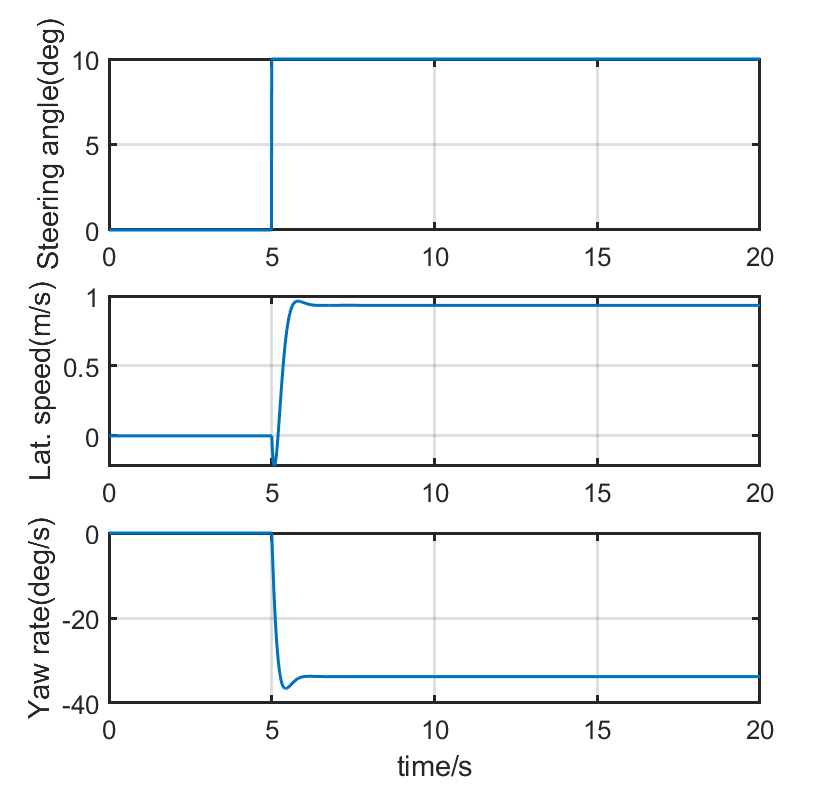
\includegraphics[width=7cm]{./figures/v20.png}
  		%\caption{Genetic Algorithm Steps}
  	\end{minipage}
  	\begin{minipage}[t]{0.45\linewidth}        %图片占用一行宽度的45%
  		\hspace{2mm}
  		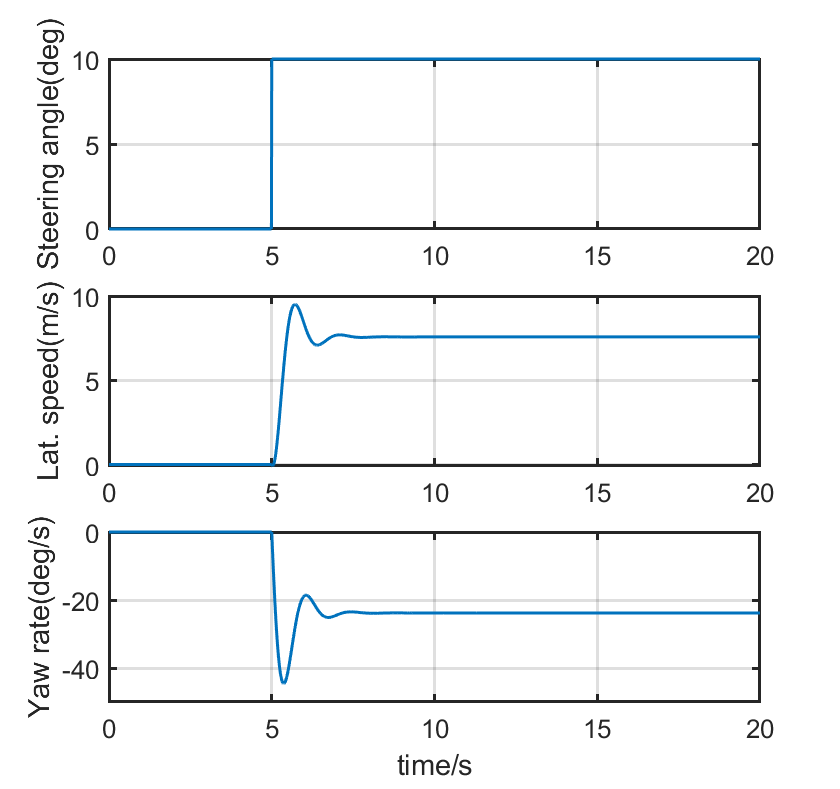
\includegraphics[width=7cm]{./figures/v50.png}
  		%\caption{Biological Principles of Genetic Algorithms}
  	\end{minipage}
  	\caption{Step response(a)$v=20m/s$(b)$v=50m/s$}
  \end{figure}

\subsection{Solution of Problem(b)}
From the bicycle model,the transient response can be written as:
\begin{equation}\label{transient}
m'\ddot{w_r} + h \dot{w_r} + c \omega _r = b_1\dot{ \delta } + b_0\delta 
\end{equation}
where \\
\begin{math}
\begin{aligned}
m' &= muI_{zz}\\
h & =-[m(a^{2} k_{1}+b^{2} k_{2})+I_{z z}(k_{1}+k_{2})] \\
c & =m u\left(a k_{1}-b k_{2}\right)-\frac{\left(a k_{1}-b k_{2}\right)^{2}}{u}+\frac{\left(k_{1}+k_{2}\right)\left(a^{2} k_{1}+b^{2} k_{2}\right)}{u} \\
& =m u\left(a k_{1}-b k_{2}\right)+\frac{L^{2} k_{1} k_{2}}{u} \\
b_{1} & =-m u a k_{1} \\
b_{0} & =L k_{1} k_{2} 
\end{aligned}
\end{math}\\
The equation \ref{transient} can be represented as:
$$
\ddot{w_r} + 2\omega_0\zeta  \dot{w_r} + \omega_0^{2} \omega _r = B_1\dot{ \delta } + B_0\delta 
$$

$$\omega_{0}=\sqrt{\frac{c}{m'}} =\frac{h}{2 \omega_{0} m'}=\frac{L}{u} \sqrt{\frac{k_{1} k_{2}}{m I_{z z}}\left(1+K u^{2}\right)} $$
$$\zeta=\frac{-m\left(a^{2} k_{1}+b^{2} k_{2}\right)-I_{z z}\left(k_{1}+k_{2}\right)}{2 L \sqrt{m I_{z z} k_{1} k_{2}\left(1+K u^{2}\right)}} $$

Natural frequency can be represented as follows:
\begin{equation}\label{omega1}
\omega_{0}= \frac{L}{u} \sqrt{\frac{k_{1} k_{2}}{m I_{z z}}\left(1+K u^{2}\right)} = L\sqrt{\frac{k_{1} k_{2}}{m I_{z z}}\left(\frac{1}{u^{2}}+K \right)}
\end{equation}

\begin{equation}\label{omega2}
\omega_{0}=\frac{L}{u} \sqrt{\frac{1}{m I_{z z}}\left[\left(\left|k_{2}\right|-\frac{m a u^{2}}{L^{2}}\right)\left|k_{1}\right|+\frac{m b u^{2}}{L^{2}}\left|k_{2}\right|\right]}
\end{equation}
\begin{itemize}
\item From equation(\ref{omega1}),it can be seen that natural frequency $\omega_0$ decrease as $u$ and $I_{zz}$ increase.
\item From equation(\ref{omega2}),it can be seen that natural frequency would be affected by the value of $\left(\left|k_{2}\right|-\frac{m a u^{2}}{L^{2}}\right)$. 
	\begin{enumerate}
	\item if $|k_2| > \frac{mau^2}{L^2}$, natural frequency $\omega_0$ will increase with increasing of $|k_1|$.
	\item if $|k_2| \le \frac{mau^2}{L^2}$,natural frequency $\omega_0$ will decrease with increasing of $|k_1|$.
	\end{enumerate}
\end{itemize}

Damping rate can be represented as follows:
\begin{equation}\label{zeta1}
\xi=\frac{-m\left(a^{2} k_{1}+b^{2} k_{2}\right)-I_{z z}\left(k_{1}+k_{2}\right)}{2 L \sqrt{m I_{z z} k_{1} k_{2}\left(1+K u^{2}\right)}}
\end{equation}

\begin{equation}\label{zeta2}
\zeta =\frac{1}{2 L \sqrt{m I_{z z} k_{1} k_{2}\left(1+K u^{2}\right)}}\left(\frac{m\left(a^{2}\left|k_{1}\right|+b^{2}\left|k_{2}\right|\right)}{\sqrt{I_{z z}}}+\sqrt{I_{z z}}\left(\left|k_{1}\right|+\left|k_{2}\right|\right)\right)
\end{equation}

\begin{itemize}
\item From equation(\ref{zeta1}),it can be seen that damping rate $\zeta$ would be affected by the value of $K$.
	\begin{enumerate}
	\item if $K > 0$,damping rate $\zeta$ will decrease with increasing of $u$
	\item if $K \le 0$,damping rate $\zeta$ will increase with increasing of $u$
	\end{enumerate}
\item From equation(\ref{zeta2}),it can be seen that natural frequency would be affected by the value of $\left(\left|k_{2}\right|-\frac{m a u^{2}}{L^{2}}\right)$. 
	\begin{enumerate}
	\item if $I_{zz} > \frac{ma^2|k_1|+b^2|k_2|}{|k_1|+|k_2|}$, damping rate $\zeta$ will increase with increasing of $I_{zz}$.
	\item if $I_{zz} \le \frac{ma^2|k_1|+b^2|k_2|}{|k_1|+|k_2|}$, damping rate $\zeta$ will decrease with increasing of $I_{zz}$.
	\end{enumerate}
\end{itemize}
 Futher,$\zeta$ takes partial derivatives with respect to $|k_1|$,we can get that $\zeta$ is an increasing function with respect to $|k_1|$. Therefore,increasing of the value of $k_1$ will lead to increasing damping rate $\zeta$.
\\Addtionally,with the help of MATLAB,we can change the input of vehicle speed $u$,moment of inertia $I_{zz}$ and front wheel concering stiffness $k_1$ respectively around the initial values and see the changes of natural frequency $\omega_0$ and damping rate $\zeta$ accordingly. All of the figures are presented in the appendix. From the figures we can validate our ideas above.

\section{Problem3}
\subsection{Problem Restatement}
\begin{itemize}
\item Derive the transfer function from the acceleration of road excitation to the acceleration of car body based on the Quarter Car Model
\item Demonstrates the changes of its bode graph with ±10\% parametric variation including $M_s,K_s,C_s$
\end{itemize}

\subsection{2DOF Quarter Car Model}
Based on the Quarter Car Model,the situation can be represented as:
\begin{equation}\label{QCM1}
M_s\ddot{x_s} + C_s(\dot{x_s} - \dot{x_u}) + K_s(x_s - x_u) = 0
\end{equation}
\begin{equation}\label{QCM2}
M_u\ddot{x_u} + C_s(\dot{x_u} - \dot{x_s}) + K_s(x_u - x_s) + C_u(\dot{x_u} - \dot{x_r}) + K_u(x_u - x_r) = 0
\end{equation}

\subsection{Solution of Problem(a)}
With the implementation of Laplace transformation on equation(\ref{QCM1}) and (\ref{QCM2}) respectively,we have the below formula,
\begin{equation}\label{laplace1}
(s^2M_s + sC_s + K_s)x_s-(sC_s + K_s)x_u = 0
\end{equation}
\begin{equation}\label{laplace2}
(s^2M_u + sC_s + K_s + sC_u + K_u)x_u - (sC_s + K_s)x_s - (sC_u + K_u)X_r = 0
\end{equation}
The relationship between $x_u$ and $x_s$ can be written as:
$$
x_u = \frac{s^2M_s + sC_s + K_s}{sC_s + K_s}x_s
$$
Substituting $x_u$ derives the transfer function from $x_r$ to $x_s$,
$$
x_{s}=\frac{\left(s C_{u}+K_{u}\right)\left(s C_{s}+K_{s}\right)}{\left[s^{4} M_{u} M_{s}+s^{2}\left(M_{s}+M_{u}\right)\left(s C_{s}+K_{s}\right)+s^{2} M_{s}\left(s C_{u}+K_{u}\right)+\left(s C_{u}+K_{u}\right)\left(s C_{s}+K_{s}\right)\right]} x_{r}
$$
Similarly,the transfer function from $\ddot{x_r}$ and $\ddot{x_s}$ can be written as:
$$
\ddot{x_{s}}=\frac{\left(s C_{u}+K_{u}\right)\left(s C_{s}+K_{s}\right)}{\left[s^{4} M_{u} M_{s}+s^{2}\left(M_{s}+M_{u}\right)\left(s C_{s}+K_{s}\right)+s^{2} M_{s}\left(s C_{u}+K_{u}\right)+\left(s C_{u}+K_{u}\right)\left(s C_{s}+K_{s}\right)\right]} \ddot{x_{r}}
$$
\subsection{Solution of Problem(b)}
With the help of MATLAB,we demonstrate the changes of the bode graph of the Quarter Car Model with $\pm 10\%$ parametric variation respectively.

\begin{figure}[h]
	\begin{minipage}{4cm}
		\centering
		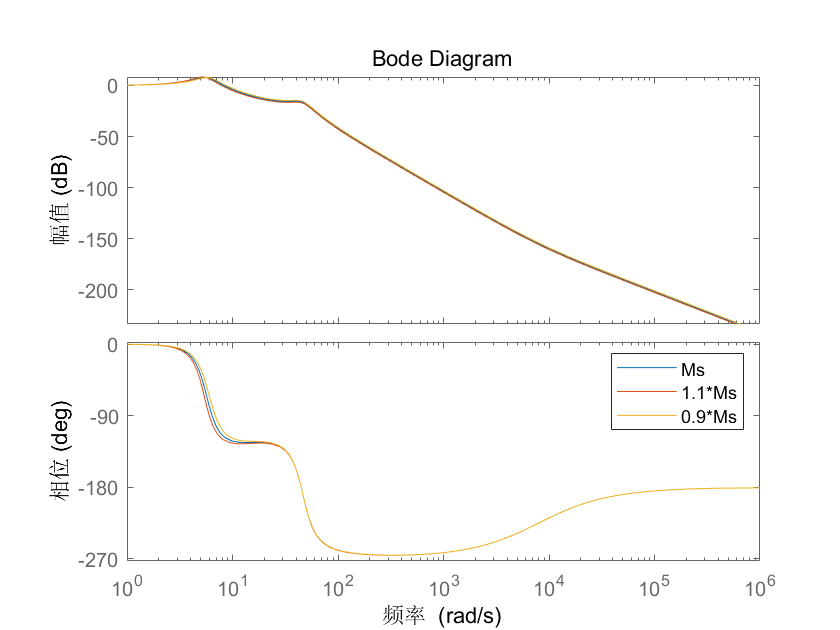
\includegraphics[width=4.5cm]{./figures/figMs.png}
		\caption{}
	\end{minipage}
	\begin{minipage}{4cm}        %图片占用一行宽度的45%
		\hspace{2mm}
		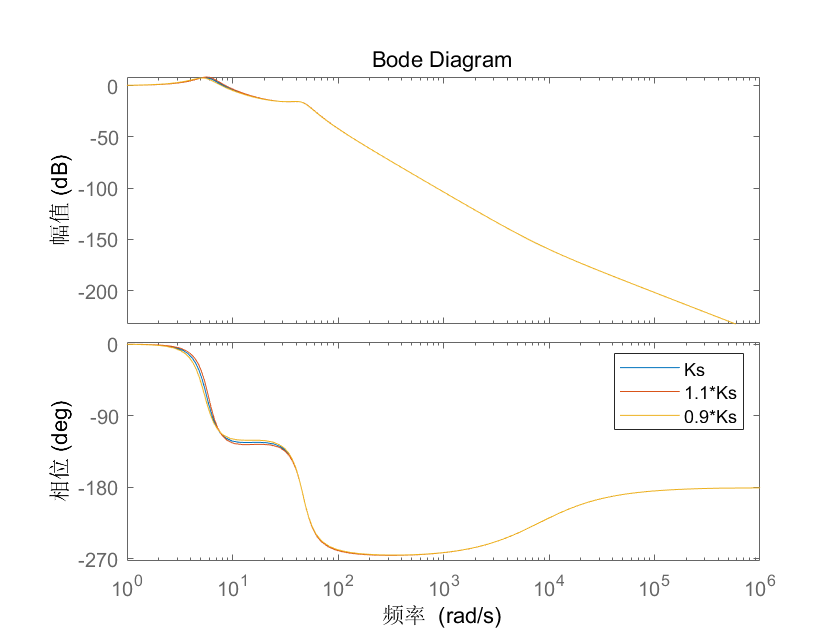
\includegraphics[width=4.5cm]{./figures/figKs.png}
		\caption{}
	\end{minipage}
	\begin{minipage}{4cm}
	\centering
	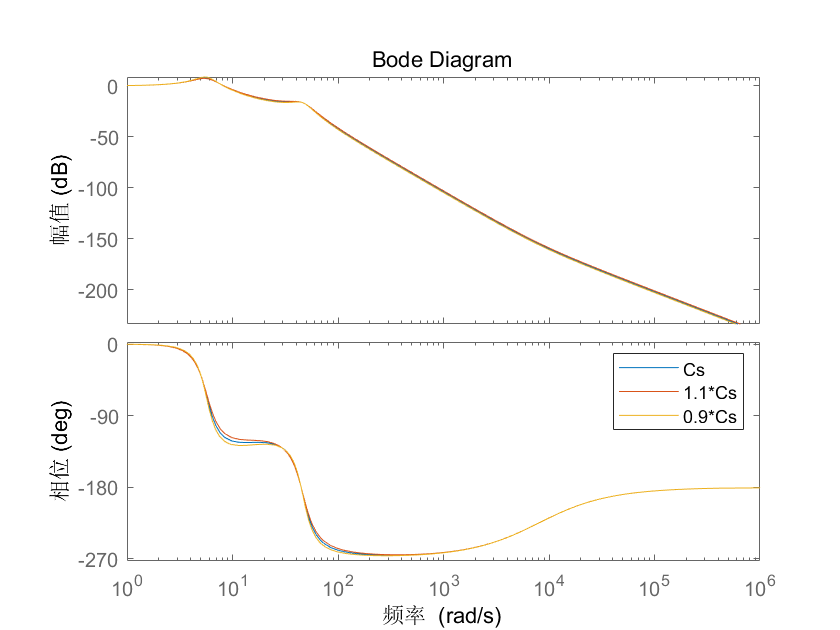
\includegraphics[width=4.5cm]{./figures/figCs.png}
	\caption{}
\end{minipage}
\caption{The bode graph  with $\pm10\%$(a)$M_s $ (b)$K_s $ (c)$ C_s$}
\end{figure}
\section{Appendix1}

\begin{figure}[htbp]
	\centering
	\subfigure[The first test of A2B]{
		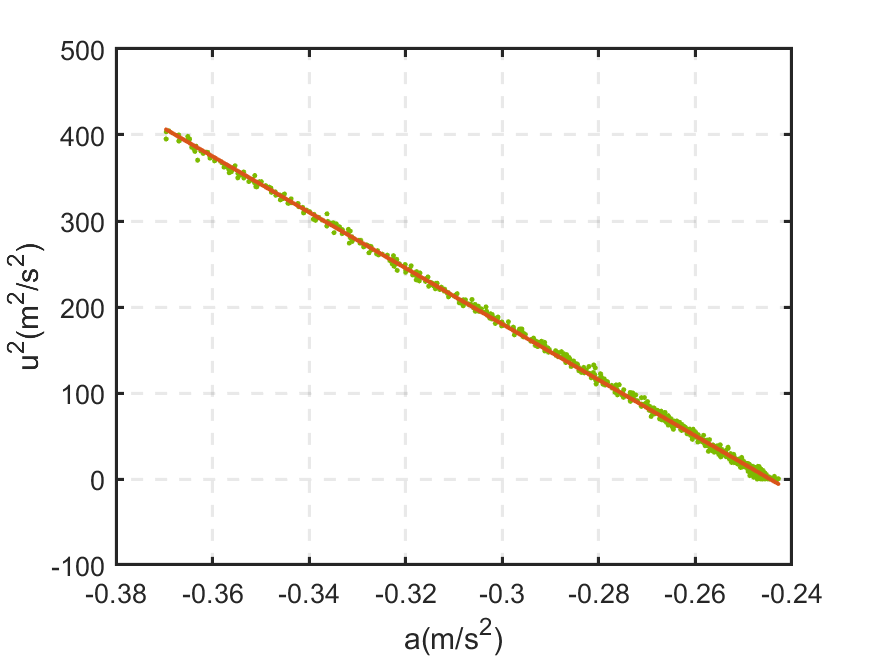
\includegraphics[width=5.5cm]{./figures/figA2B_1.png}
		%\caption{fig1}
	}
	\quad
	\subfigure[The second test of A2B]{
		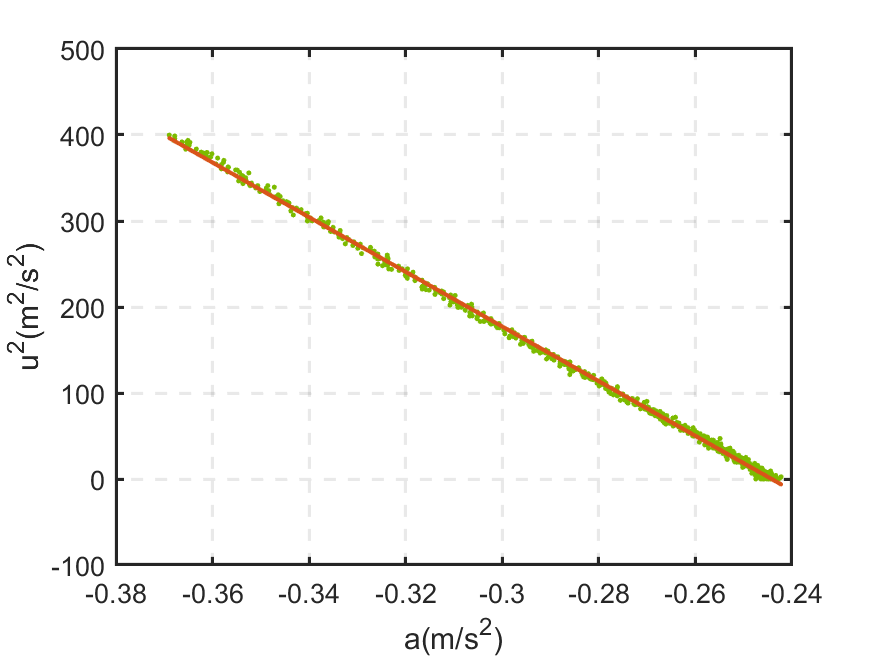
\includegraphics[width=5.5cm]{./figures/figA2B_2.png}
	}
	\quad
	\subfigure[The third test of A2B]{
		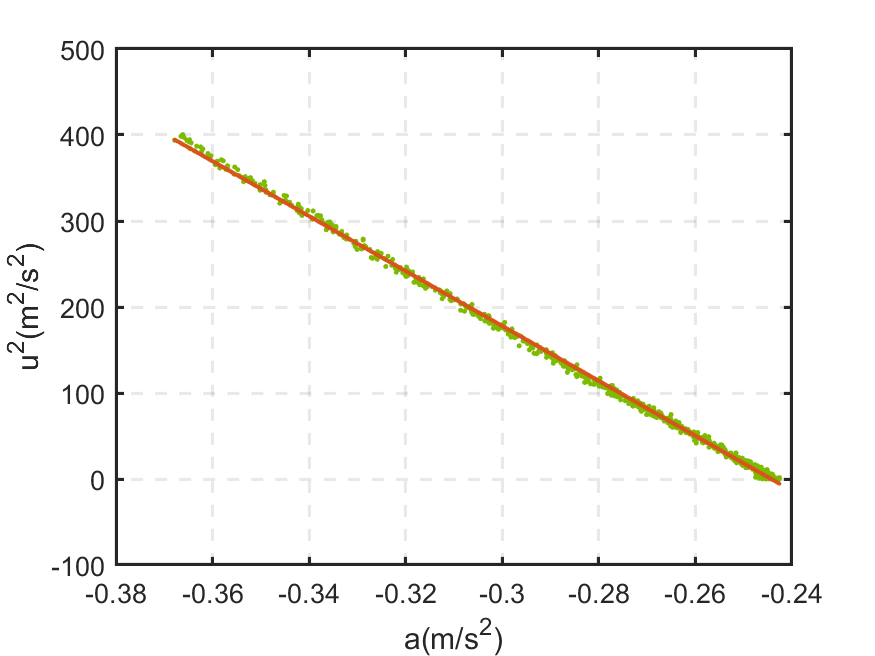
\includegraphics[width=5.5cm]{./figures/figA2B_3}
	}
	\quad
	\subfigure[The fourth test of A2B]{
		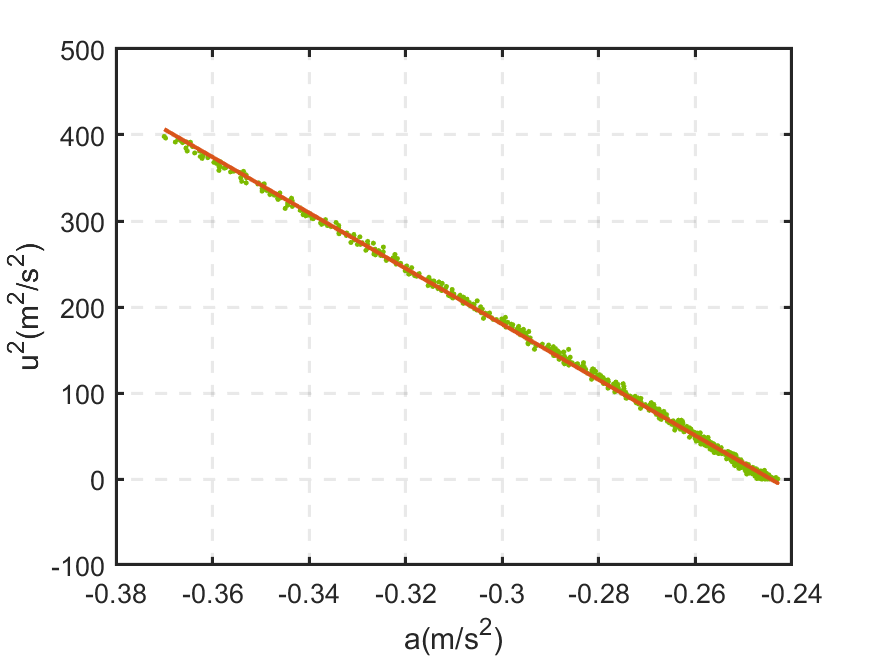
\includegraphics[width=5.5cm]{./figures/figA2B_4}
	}
	\caption{The fitting of test A2B}
\end{figure}
\begin{figure}[htbp]
	\centering
	\subfigure[The first test of B2A]{
		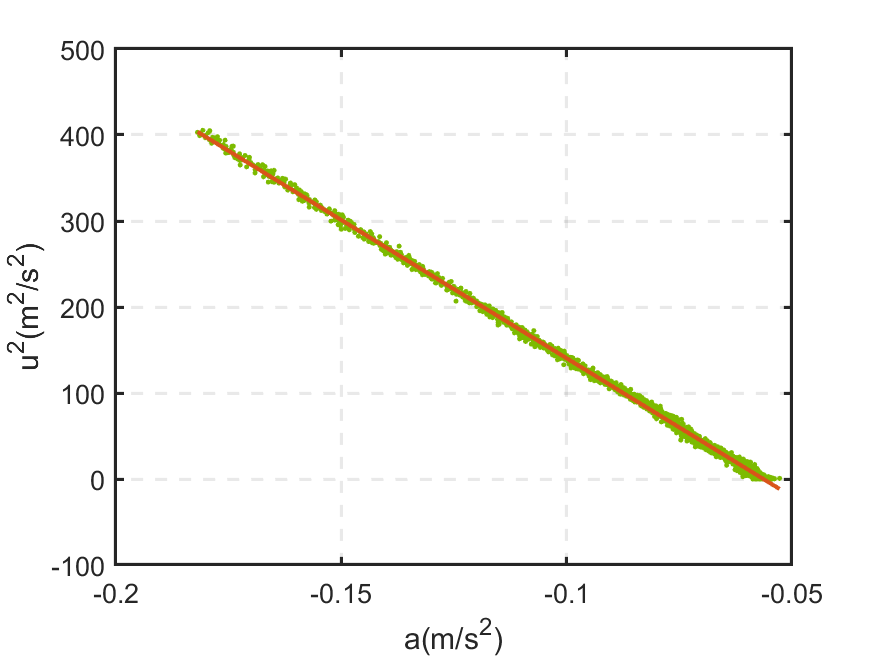
\includegraphics[width=5.5cm]{./figures/figB2A_1.png}
		%\caption{fig1}
	}
	\quad
	\subfigure[The second test of B2A]{
		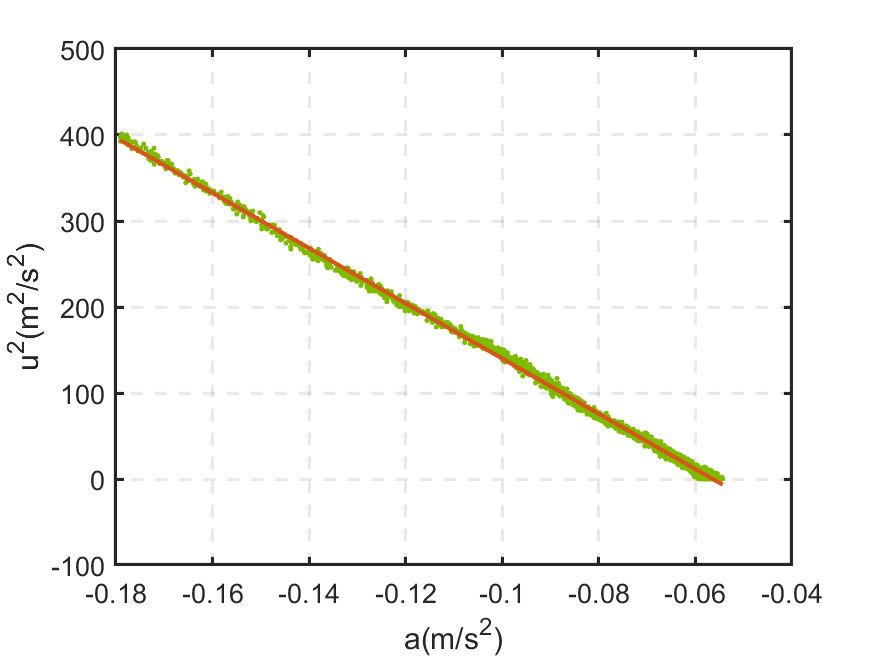
\includegraphics[width=5.5cm]{./figures/figB2A_2.png}
	}
	\quad
	\subfigure[The third test of B2A]{
		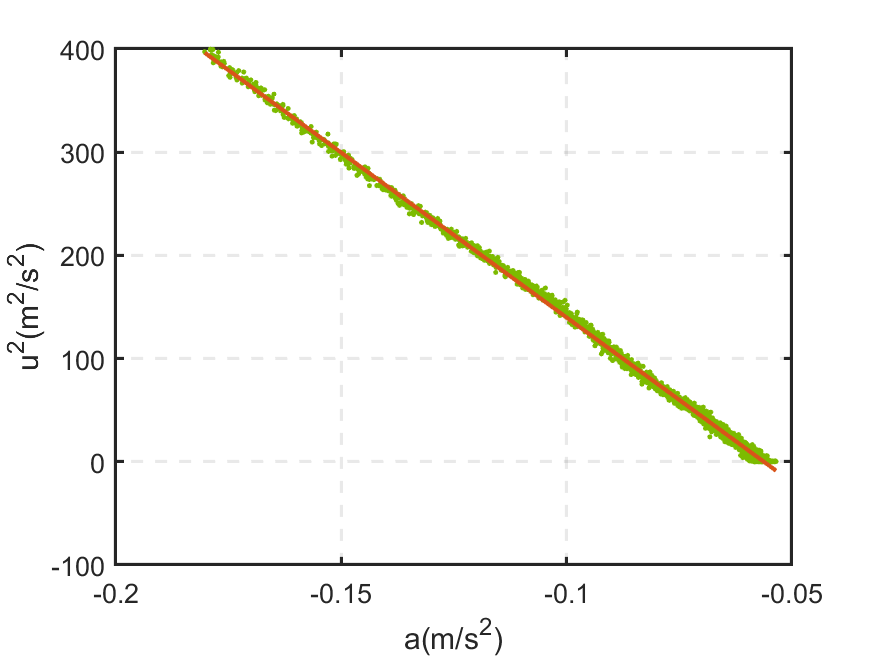
\includegraphics[width=5.5cm]{./figures/figB2A_3}
	}
	\quad
	\subfigure[The fourth test of B2A]{
		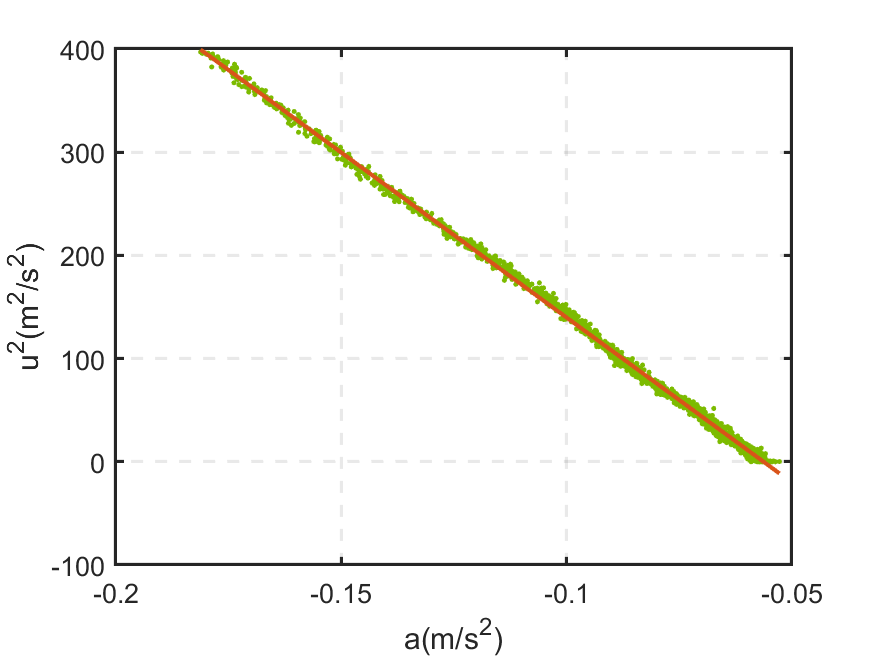
\includegraphics[width=5.5cm]{./figures/figB2A_4}
	}
	\caption{The fitting of test B2A}
\end{figure}
\newpage
\section{Appendix2}
\begin{figure}[h]
	\begin{minipage}{4.5cm}
		\centering
		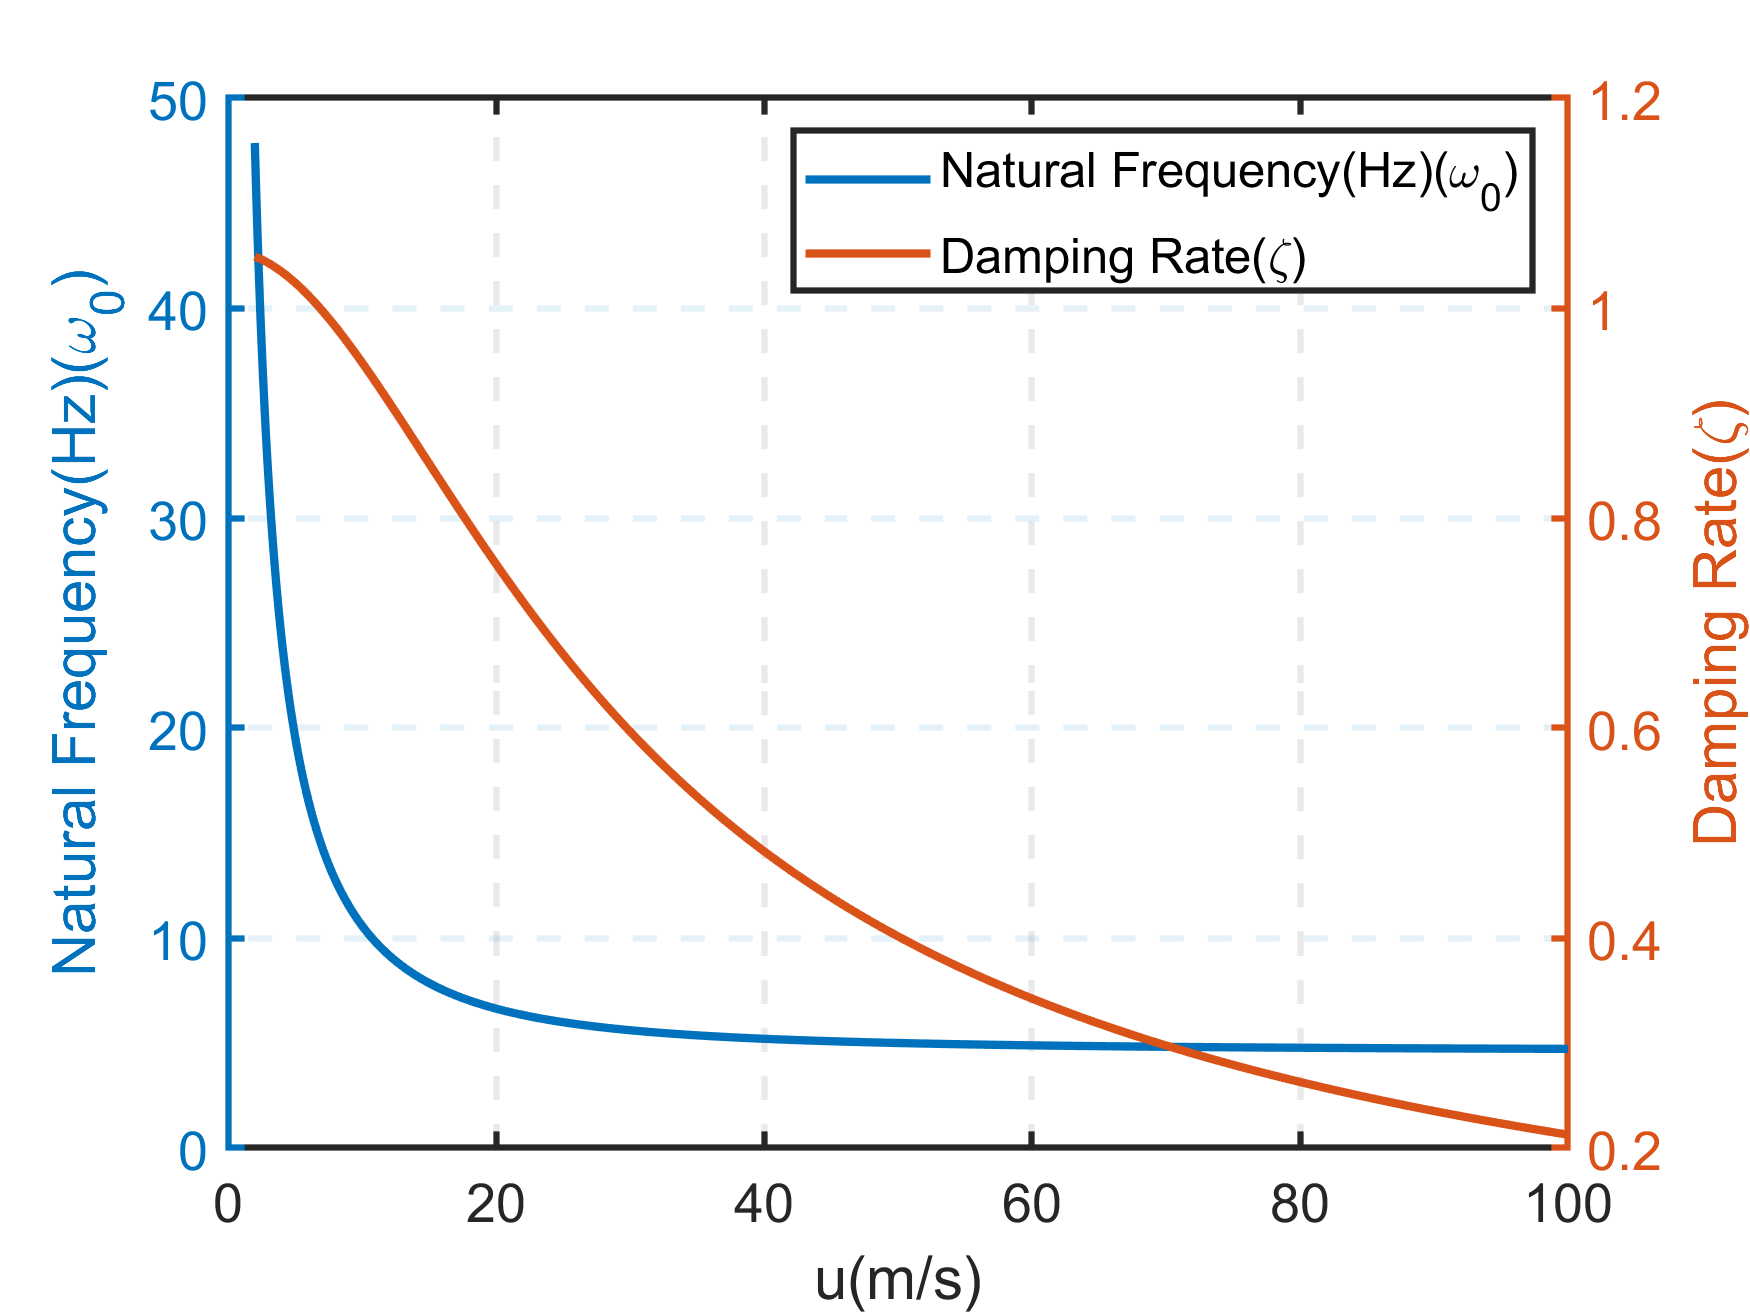
\includegraphics[width=4.5cm]{./figures/figu-nf-dr.png}
		\caption{}
	\end{minipage}
	\begin{minipage}{4.5cm}        %图片占用一行宽度的45%
		\hspace{2mm}
		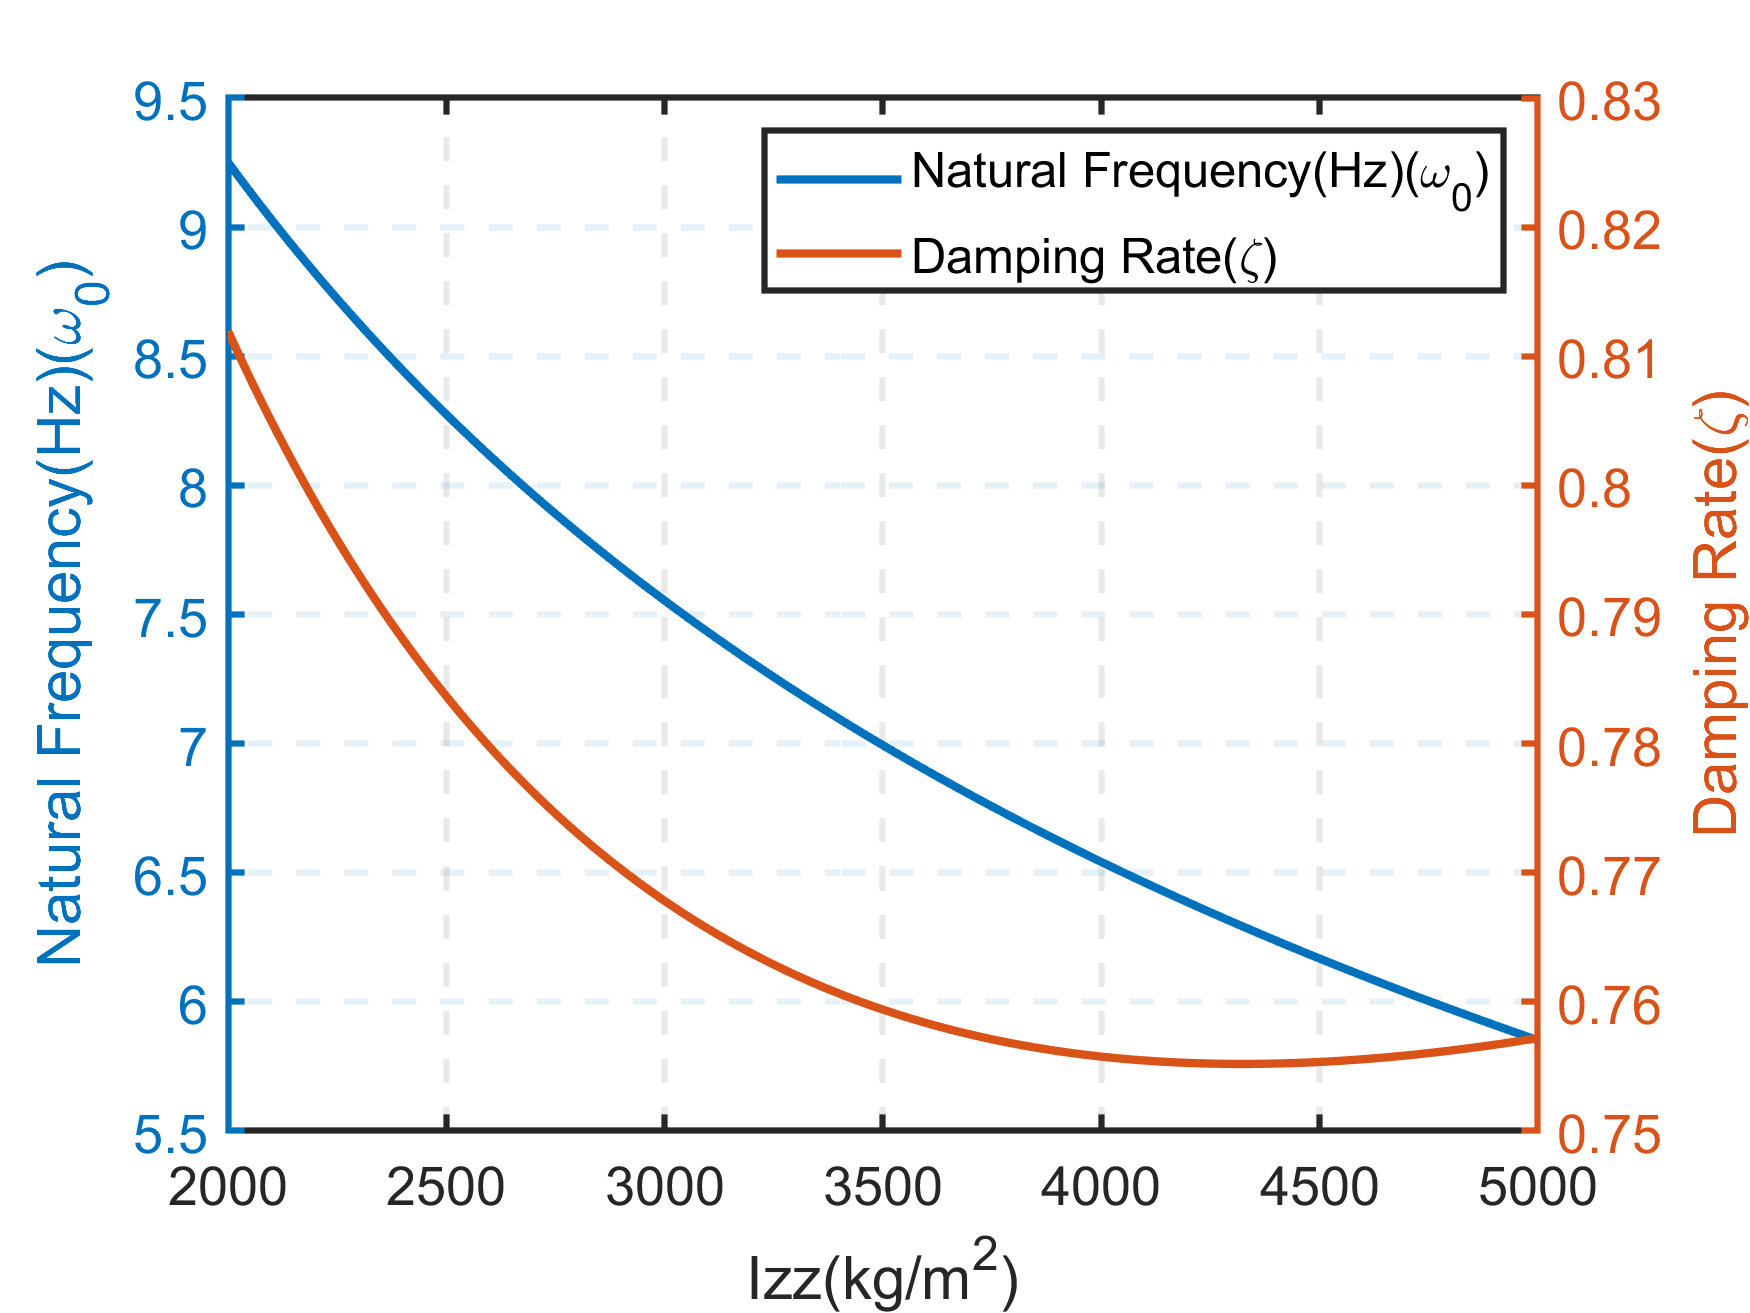
\includegraphics[width=4.5cm]{./figures/figI-nf-dr.png}
		\caption{}
	\end{minipage}
	\begin{minipage}{4.5cm}
	\centering
	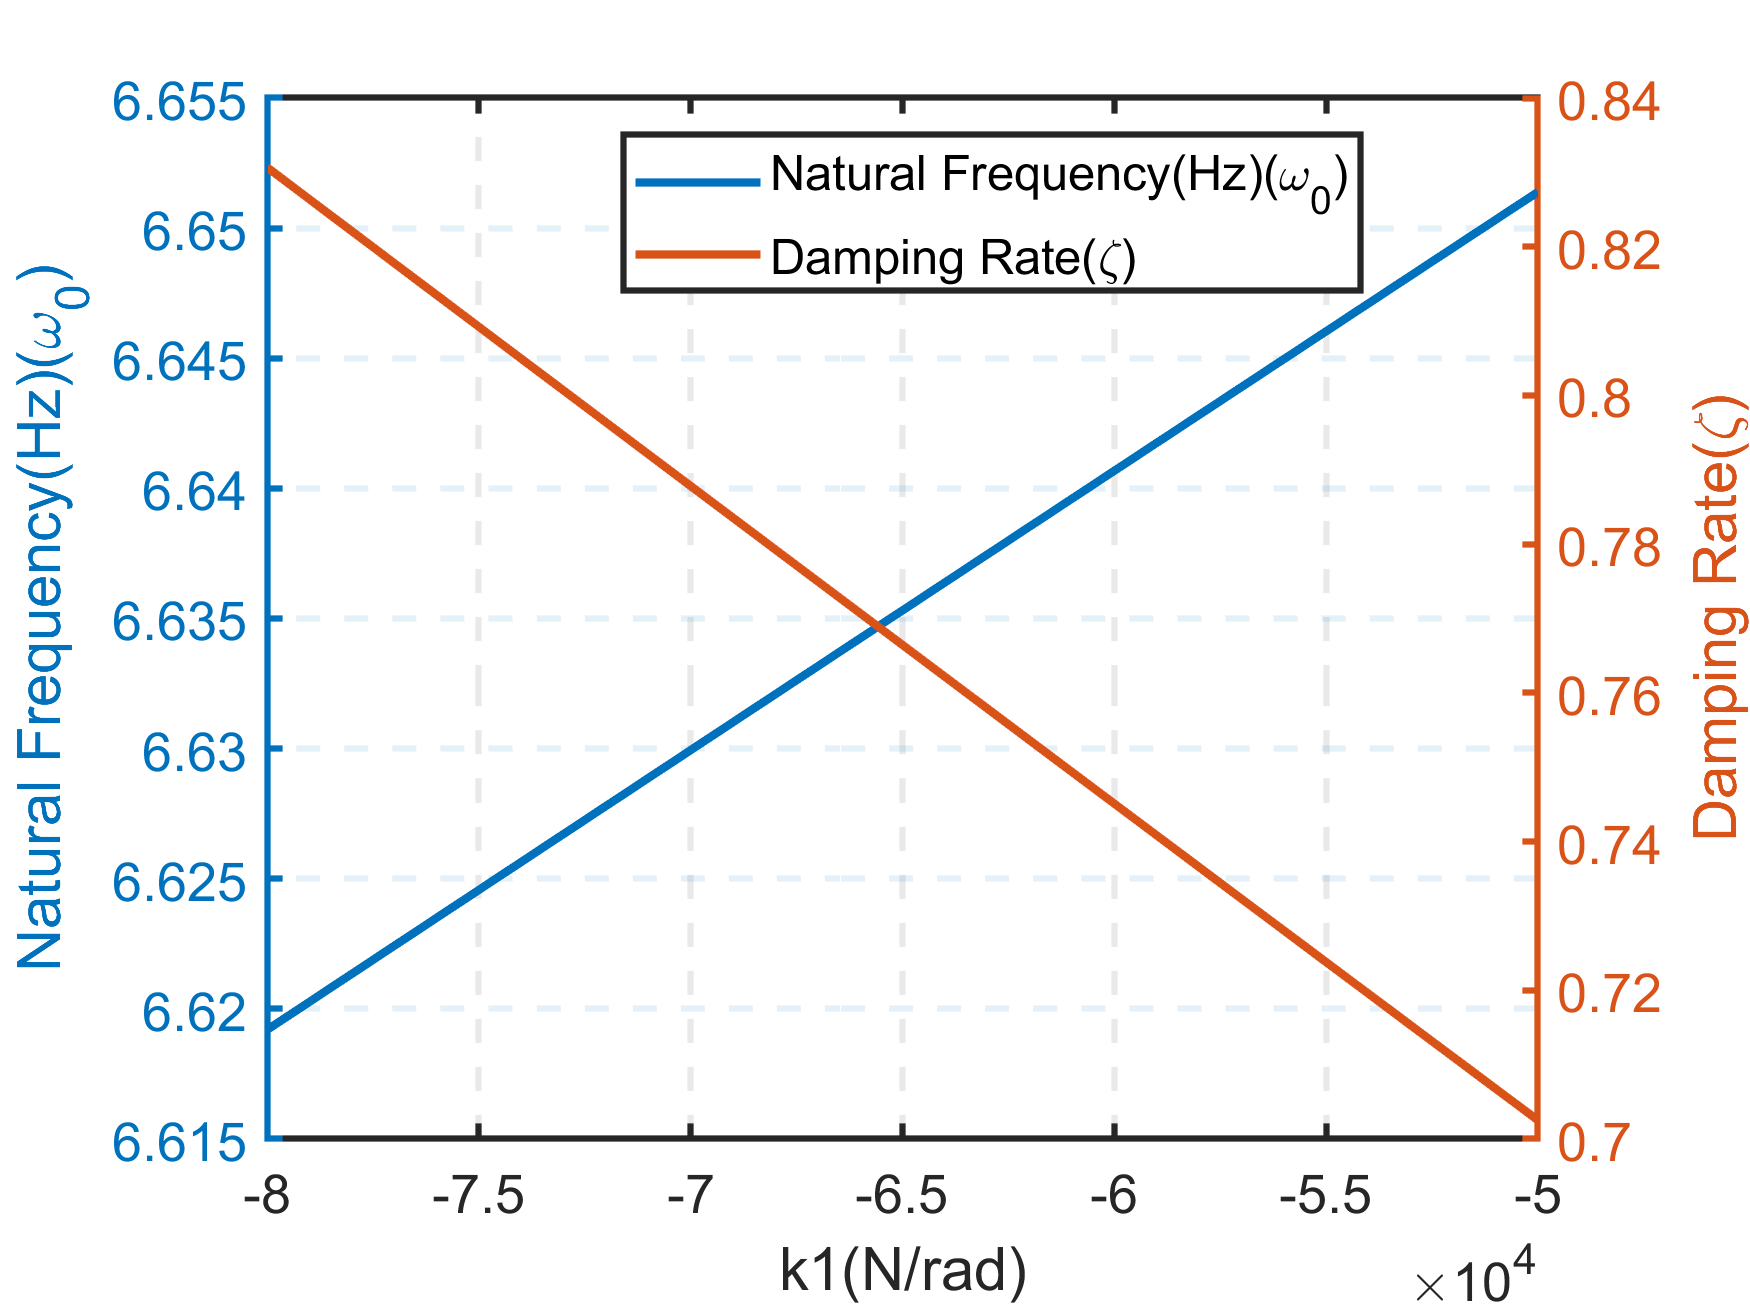
\includegraphics[width=4.5cm]{./figures/figk1-nf-dr.png}
	\caption{}
\end{minipage}
\caption{The relationship between $u$,$I_{zz}$,$k_1$ and $\omega_0$,$\zeta$}
\end{figure}

\end{document}